\documentclass[notes,11pt, aspectratio=169, xcolor=table]{beamer}

\usepackage{pgfpages}
% These slides also contain speaker notes. You can print just the slides,
% just the notes, or both, depending on the setting below. Comment out the want
% you want.
\setbeameroption{hide notes} % Only slide
%\setbeameroption{show only notes} % Only notes
%\setbeameroption{show notes on second screen=right} % Both


\newtheorem{proposition}{Proposition}
\newcommand{\blue}[1]{\textcolor{blue}{#1}}
\newcommand{\white}[1]{\textcolor{white}{#1}}

\usepackage{helvet}
\usepackage[default]{lato}
\usepackage{array}
\usepackage{tikz}
\usetikzlibrary{shapes.geometric}
\usepackage{pgfplots}
\usetikzlibrary{patterns, pgfplots.fillbetween}
\usepackage{graphicx}
\usepackage{verbatim}
\setbeamertemplate{note page}{\pagecolor{yellow!5}\insertnote}
\usetikzlibrary{positioning}
\usetikzlibrary{snakes}
\usetikzlibrary{calc}
\usetikzlibrary{arrows}
\usetikzlibrary{decorations.markings}
\usetikzlibrary{shapes.misc}
\usetikzlibrary{matrix,shapes,arrows,fit,tikzmark}
\usepackage{amsmath}
\usepackage{mathpazo}
\usepackage{hyperref}
\usepackage{lipsum}
\usepackage{multimedia}
\usepackage{graphicx}
\usepackage{multirow}
\usepackage{graphicx}
\usepackage{dcolumn}
\usepackage{bbm}
\usepackage[style=authoryear,sorting=nyt,uniquename=false]{biblatex}

\addbibresource{references.bib} 

\newcolumntype{d}[0]{D{.}{.}{5}}

\def\@@mybluebox[#1][#2]#3{
    \sbox\mytempbox{#3}%
    \mytemplen\ht\mytempbox
    \advance\mytemplen #1\relax
    \ht\mytempbox\mytemplen
    \mytemplen\dp\mytempbox
    \advance\mytemplen #2\relax
    \dp\mytempbox\mytemplen
    \colorbox{myblue}{\hspace{1em}\usebox{\mytempbox}\hspace{1em}}}


\usepackage{changepage}
\usepackage{appendixnumberbeamer}
\newcommand{\beginbackup}{
   \newcounter{framenumbervorappendix}
   \setcounter{framenumbervorappendix}{\value{framenumber}}
   \setbeamertemplate{footline}
   {
     \leavevmode%
     \hline
     box{%
       \begin{beamercolorbox}[wd=\paperwidth,ht=2.25ex,dp=1ex,right]{footlinecolor}%
%         \insertframenumber  \hspace*{2ex} 
       \end{beamercolorbox}}%
     \vskip0pt%
   }
 }
\newcommand{\backupend}{
   \addtocounter{framenumbervorappendix}{-\value{framenumber}}
   \addtocounter{framenumber}{\value{framenumbervorappendix}} 
}


\usepackage{graphicx}
\usepackage[space]{grffile}
\usepackage{booktabs}

% These are my colors -- there are many like them, but these ones are mine.
\definecolor{blue}{RGB}{0,114,178}
\definecolor{red}{RGB}{213,94,0}
\definecolor{yellow}{RGB}{240,228,66}
\definecolor{green}{RGB}{0,158,115}

\hypersetup{
  colorlinks=false,
  linkbordercolor = {white},
  linkcolor = {blue}
}


%% I use a beige off white for my background
\definecolor{MyBackground}{RGB}{255,253,218}

%% Uncomment this if you want to change the background color to something else
%\setbeamercolor{background canvas}{bg=MyBackground}

%% Change the bg color to adjust your transition slide background color!
\newenvironment{transitionframe}{
  \setbeamercolor{background canvas}{bg=yellow}
  \begin{frame}}{
    \end{frame}
}

\setbeamercolor{frametitle}{fg=blue}
\setbeamercolor{title}{fg=blue}
\setbeamertemplate{footline}[frame number]
\setbeamertemplate{navigation symbols}{} 
\setbeamertemplate{itemize items}{-}
\setbeamercolor{itemize item}{fg=blue}
\setbeamercolor{itemize subitem}{fg=blue}
\setbeamercolor{enumerate item}{fg=blue}
\setbeamercolor{enumerate subitem}{fg=blue}
\setbeamercolor{button}{bg=MyBackground,fg=blue,}



% If you like road maps, rather than having clutter at the top, have a roadmap show up at the end of each section 
% (and after your introduction)
% Uncomment this is if you want the roadmap!
% \AtBeginSection[]
% {
%    \begin{frame}
%        \frametitle{Roadmap of Talk}
%        \tableofcontents[currentsection]
%    \end{frame}
% }
\setbeamercolor{section in toc}{fg=blue}
\setbeamercolor{subsection in toc}{fg=red}
\setbeamersize{text margin left=1em,text margin right=1em} 

\newenvironment{wideitemize}{\itemize\addtolength{\itemsep}{10pt}}{\enditemize}

\usepackage{environ}
\NewEnviron{videoframe}[1]{
  \begin{frame}
    \vspace{-8pt}
    \begin{columns}[onlytextwidth, T] % align columns
      \begin{column}{.58\textwidth}
        \begin{minipage}[t][\textheight][t]
          {\dimexpr\textwidth}
          \vspace{8pt}
          \hspace{4pt} {\Large \sc \textcolor{blue}{#1}}
          \vspace{8pt}
          
          \BODY
        \end{minipage}
      \end{column}%
      \hfill%
      \begin{column}{.42\textwidth}
        \colorbox{green!20}{\begin{minipage}[t][1.2\textheight][t]
            {\dimexpr\textwidth}
            Face goes here
          \end{minipage}}
      \end{column}%
    \end{columns}
  \end{frame}
}

\title[]{International Trade: Lecture 13}
\subtitle[]{The Standard Trade Model, Gravity, and Welfare}
\author[Góes]
{Carlos Góes\inst{1}}
\date{Fall 2025}
\institute[GWU]{\inst{1} George Washington University }



\begin{document}

%%% TIKZ STUFF
\tikzset{   
        every picture/.style={remember picture,baseline},
        every node/.style={anchor=base,align=center,outer sep=1.5pt},
        every path/.style={thick},
        }
\newcommand\marktopleft[1]{%
    \tikz[overlay,remember picture] 
        \node (marker-#1-a) at (-.3em,.3em) {};%
}
\newcommand\markbottomright[2]{%
    \tikz[overlay,remember picture] 
        \node (marker-#1-b) at (0em,0em) {};%
}
\tikzstyle{every picture}+=[remember picture] 
\tikzstyle{mybox} =[draw=black, very thick, rectangle, inner sep=10pt, inner ysep=20pt]
\tikzstyle{fancytitle} =[draw=black,fill=red, text=white]
%%%% END TIKZ STUFF



%----------------------------------------------------------------------%
%-------------------       TITLE PAGE       ---------------------------%
%----------------------------------------------------------------------%





%----------------------------------------------------------------------%






%----------------------------------------------------------------------%
%----------------------------------------------------------------------%

%----------------------------------------------------------------------%
\frame{\titlepage}
\addtocounter{framenumber}{-1}
%----------------------------------------------------------------------%



%----------------------------------------------------------------------%
%----------------------------------------------------------------------%

\section{Intro and recap}

\begin{frame}{So far\ldots}
\begin{wideitemize}
  \item \blue{Ricardian:} differences in technology induce comparative advantage; constant returns
  \item<2-> \blue{Specific-Factors:} specific factors $\rightarrow$ decreasing returns $\rightarrow$ distributional effects
  \item<3-> \blue{Heckscher–Ohlin:} same tech, different endowments $\rightarrow$ patterns of specialization
  \item<4-> \blue{Standard Trade Model:} trade happens due to differences $\rightarrow$ changes in terms of trade 
\end{wideitemize}
\end{frame}

\begin{frame}{This class}
\begin{wideitemize}
    \item Welfare gains from trade across models
    \item Changes in Terms of Trade (ToT) + growth bias 
    \item The Gravity Equation
    \item Empirical estimates of welfare gains
    \item Data Lab will go hands-on later.
\end{wideitemize}
\end{frame}

\section{The Standard Trade Model}


\begin{frame}{Graphical representation}

\begin{columns}[T] % align columns
\begin{column}{.4\textwidth}
            \centering
    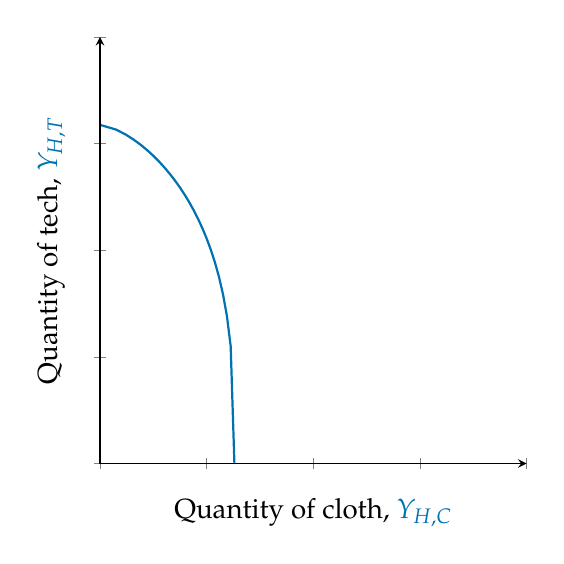
\begin{tikzpicture}
    \pgfmathsetmacro{\alpha}{0.5}
    \pgfmathsetmacro{\betat}{2/3}
    \pgfmathsetmacro{\betac}{1/3}

    \pgfmathsetmacro{\Phi}{((1-\betat)^(1-\betat))*((\betat)^\betat)/
             ((1-\betac)^(1-\betac))*((\betac)^\betac)}
    \pgfmathsetmacro{\aC}{\betac/(1-\betac)}
    \pgfmathsetmacro{\aT}{\betat/(1-\betat)}
    \pgfmathsetmacro{\d}{\aC-\aT}

    
    \pgfmathsetmacro{\L}{1}
    \pgfmathsetmacro{\K}{2.25}
    \pgfmathsetmacro{\Kk}{1.5}

   \pgfmathsetmacro{\wra}{ \K / \L * (\alpha*(1-\betac) + (1-\alpha)*(1-\betat))/(\alpha * \betac + (1-\alpha)*\betat)  }
    \pgfmathsetmacro{\wr}{  \Kk / \L * (\alpha*(1-\betac) + (1-\alpha)*(1-\betat))/(\alpha * \betac + (1-\alpha)*\betat) }

    \pgfmathsetmacro{\P}{ ( ((1-\betat)^(1-\betat) * \betat^(\betat)) / ((1-\betac)^(1-\betac) * \betac^(\betac)) ) * (\wr)^(\betat-\betac)  }

       
    \pgfmathsetmacro{\Lc}{ (\K - \aT*\wr*\L)/(\d * \wr) }
    \pgfmathsetmacro{\Kc}{\aC * \wr * \Lc}
    \pgfmathsetmacro{\Lt}{\L - \Lc}
    \pgfmathsetmacro{\Kt}{\K - \Kc}
   
    \pgfmathsetmacro{\Yc}{ \Kc^(\betac) * \Lc^(1-\betac) }
    \pgfmathsetmacro{\Yt}{ \Kt^(\betat) * \Lt^(1-\betat) }

    

    \pgfmathsetmacro{\I}{ \P * \Yc + \Yt }
    \pgfmathsetmacro{\Qc}{(1-\alpha)/\P * \I}
    \pgfmathsetmacro{\Qt}{(\alpha) * \I}

    \pgfmathsetmacro{\U}{(\Qt^(\alpha))*(\Qc^(1 - \alpha))}
    \pgfmathsetmacro{\expo}{(1 - \alpha)/\alpha}
    \pgfmathsetmacro{\A}{\U^(1/\alpha)}

    
    
    \centering
    \begin{axis}[
        ylabel={Quantity of tech, $\textcolor{blue}{Y_{H,T}}$},
        xlabel={Quantity of cloth, $\textcolor{blue}{Y_{H,C}}$},
        ymin=0, ymax=2,
        xmin=0, xmax=2,
        yticklabel=\empty,
        xticklabel=\empty,
        axis lines=left,
        enlargelimits=false,
        clip=false,
        axis on top,
        scaled x ticks=false,
        width=7cm, height=7cm,
        title style={font=\bfseries}
    ]
    
    % PPF: Q_C = (L/a_C) - (a_R/a_C) * Q_R
    \addplot[blue, thick, domain=0:1] ({ \Kc^(\betac) * (\L-x)^(1-\betac)}, { \Kt^(\betat) * (x)^(1-\betat)});
    

        

    
    \end{axis}

\end{tikzpicture}

                
    \end{column}
    \begin{column}{.45\textwidth}

    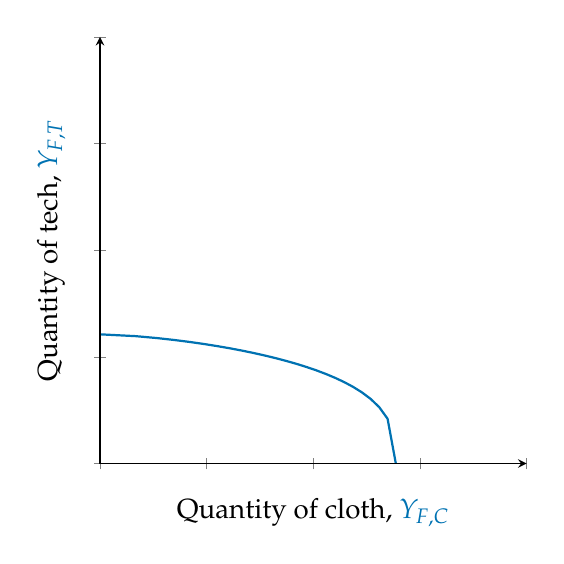
\begin{tikzpicture}
    \pgfmathsetmacro{\alpha}{0.5}
    \pgfmathsetmacro{\betat}{2/3}
    \pgfmathsetmacro{\betac}{1/3}

    \pgfmathsetmacro{\Phi}{((1-\betat)^(1-\betat))*((\betat)^\betat)/
             ((1-\betac)^(1-\betac))*((\betac)^\betac)}
    \pgfmathsetmacro{\aC}{\betac/(1-\betac)}
    \pgfmathsetmacro{\aT}{\betat/(1-\betat)}
    \pgfmathsetmacro{\d}{\aC-\aT}

    
    \pgfmathsetmacro{\L}{2}
    \pgfmathsetmacro{\K}{1}
    \pgfmathsetmacro{\Kk}{1.5}

   \pgfmathsetmacro{\wra}{ \K / \L * (\alpha*(1-\betac) + (1-\alpha)*(1-\betat))/(\alpha * \betac + (1-\alpha)*\betat)  }
    \pgfmathsetmacro{\wr}{  \Kk / \L * (\alpha*(1-\betac) + (1-\alpha)*(1-\betat))/(\alpha * \betac + (1-\alpha)*\betat) }

    \pgfmathsetmacro{\P}{ ( ((1-\betat)^(1-\betat) * \betat^(\betat)) / ((1-\betac)^(1-\betac) * \betac^(\betac)) ) * (\wr)^(\betat-\betac)  }

       
    \pgfmathsetmacro{\Lc}{ (\K - \aT*\wr*\L)/(\d * \wr) }
    \pgfmathsetmacro{\Kc}{\aC * \wr * \Lc}
    \pgfmathsetmacro{\Lt}{\L - \Lc}
    \pgfmathsetmacro{\Kt}{\K - \Kc}
   
    \pgfmathsetmacro{\Yc}{ \Kc^(\betac) * \Lc^(1-\betac) }
    \pgfmathsetmacro{\Yt}{ \Kt^(\betat) * \Lt^(1-\betat) }

    

    \pgfmathsetmacro{\I}{ \P * \Yc + \Yt }
    \pgfmathsetmacro{\Qc}{(1-\alpha)/\P * \I}
    \pgfmathsetmacro{\Qt}{(\alpha) * \I}

    \pgfmathsetmacro{\U}{(\Qt^(\alpha))*(\Qc^(1 - \alpha))}
    \pgfmathsetmacro{\expo}{(1 - \alpha)/\alpha}
    \pgfmathsetmacro{\A}{\U^(1/\alpha)}

    
    
    \centering
    \begin{axis}[
        ylabel={Quantity of tech, $\textcolor{blue}{Y_{F,T}}$},
        xlabel={Quantity of cloth, $\textcolor{blue}{Y_{F,C}}$},
        ymin=0, ymax=2,
        xmin=0, xmax=2,
        yticklabel=\empty,
        xticklabel=\empty,
        axis lines=left,
        enlargelimits=false,
        clip=false,
        axis on top,
        scaled x ticks=false,
        width=7cm, height=7cm,
        title style={font=\bfseries}
    ]
    
    % PPF: Q_C = (L/a_C) - (a_R/a_C) * Q_R
    \addplot[blue, thick, domain=0:2] ({ \Kc^(\betac) * (\L-x)^(1-\betac)}, { \Kt^(\betat) * (x)^(1-\betat)});
    



    
    \end{axis}

\end{tikzpicture}

    \end{column}
\end{columns}
\end{frame}


\begin{frame}{Graphical representation}
\addtocounter{framenumber}{-1}

\begin{columns}[T] % align columns
\begin{column}{.4\textwidth}
            \centering
    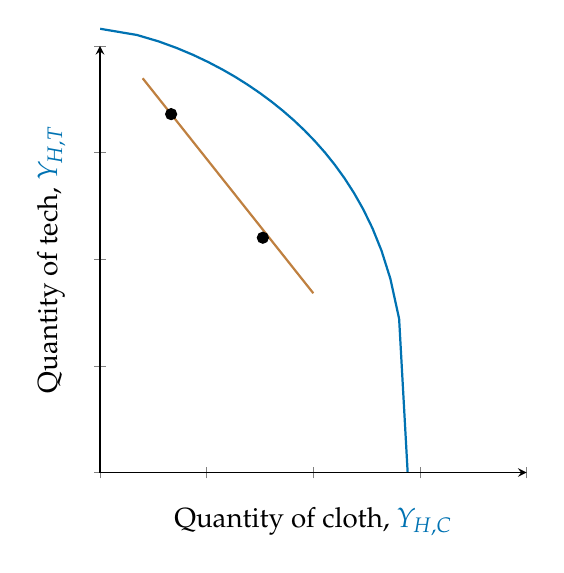
\begin{tikzpicture}
    \pgfmathsetmacro{\alpha}{0.5}
    \pgfmathsetmacro{\betat}{2/3}
    \pgfmathsetmacro{\betac}{1/3}

    \pgfmathsetmacro{\Phi}{((1-\betat)^(1-\betat))*((\betat)^\betat)/
             ((1-\betac)^(1-\betac))*((\betac)^\betac)}
    \pgfmathsetmacro{\aC}{\betac/(1-\betac)}
    \pgfmathsetmacro{\aT}{\betat/(1-\betat)}
    \pgfmathsetmacro{\d}{\aC-\aT}

    
    \pgfmathsetmacro{\L}{1}
    \pgfmathsetmacro{\K}{3}
    \pgfmathsetmacro{\Kk}{2}

   \pgfmathsetmacro{\wra}{ \K / \L * (\alpha*(1-\betac) + (1-\alpha)*(1-\betat))/(\alpha * \betac + (1-\alpha)*\betat)  }
    \pgfmathsetmacro{\wr}{  \Kk / \L * (\alpha*(1-\betac) + (1-\alpha)*(1-\betat))/(\alpha * \betac + (1-\alpha)*\betat) }

    \pgfmathsetmacro{\P}{ ( ((1-\betat)^(1-\betat) * \betat^(\betat)) / ((1-\betac)^(1-\betac) * \betac^(\betac)) ) * (\wr)^(\betat-\betac)  }
    \pgfmathsetmacro{\Pa}{ ( ((1-\betat)^(1-\betat) * \betat^(\betat)) / ((1-\betac)^(1-\betac) * \betac^(\betac)) ) * (\wra)^(\betat-\betac)  }

       
    \pgfmathsetmacro{\Lc}{ (\K - \aT*\wr*\L)/(\d * \wr) }
    \pgfmathsetmacro{\Kc}{\aC * \wr * \Lc}
    \pgfmathsetmacro{\Lt}{\L - \Lc}
    \pgfmathsetmacro{\Kt}{\K - \Kc}
   
    \pgfmathsetmacro{\Yc}{ \Kc^(\betac) * \Lc^(1-\betac) }
    \pgfmathsetmacro{\Yt}{ \Kt^(\betat) * \Lt^(1-\betat) }

    \pgfmathsetmacro{\Lca}{ (\K - \aT*\wra*\L)/(\d * \wra) }
    \pgfmathsetmacro{\Kca}{\aC * \wra * \Lca}
    \pgfmathsetmacro{\Lta}{\L - \Lca}
    \pgfmathsetmacro{\Kta}{\K - \Kca}
   
    \pgfmathsetmacro{\Yca}{ \Kca^(\betac) * \Lca^(1-\betac) }
    \pgfmathsetmacro{\Yta}{ \Kta^(\betat) * \Lta^(1-\betat) }

    
    
    \centering
    \begin{axis}[
        ylabel={Quantity of tech, $\textcolor{blue}{Y_{H,T}}$},
        xlabel={Quantity of cloth, $\textcolor{blue}{Y_{H,C}}$},
        ymin=0, ymax=2,
        xmin=0, xmax=2,
        yticklabel=\empty,
        xticklabel=\empty,
        axis lines=left,
        enlargelimits=false,
        clip=false,
        axis on top,
        scaled x ticks=false,
        width=7cm, height=7cm,
        title style={font=\bfseries}
    ]
    
    % PPF: Q_C = (L/a_C) - (a_R/a_C) * Q_R
    \addplot[blue, thick, domain=0:1] ({ \K^(\betac) * (\L-x)^(1-\betac)}, { \K^(\betat) * (x)^(1-\betat)});
    \pgfmathsetmacro{\c}{ \Yt + \P * \Yc }
    \addplot[thick, brown, domain=0.2:1] { \c - \P*x};

    %\pgfmathsetmacro{\ck}{ \Ytk + \Pk * \Yck }
    %\addplot[thick, brown, domain=0.2:1] { \ck - \Pk*x};


    % Equilibrium point
    \addplot[only marks, mark=*, color=black, mark size=2pt] coordinates {(\Yc, \Yt)};
    %\node[anchor = north east] at (axis cs:\Yc,\Yt) {\scriptsize Production};
    %\node[anchor = east] at (axis cs:\Yc,\Yt) {\scriptsize $(Y_{H,C},Y_{H,T})$};

    % Equilibrium point
    \addplot[only marks, mark=*, color=black, mark size=2pt] coordinates {(\Yca, \Yta)};
%    \node[anchor = north east] at (axis cs:\Yc,\Yt) {\scriptsize Production};
%    \node[anchor = east] at (axis cs:\Yc,\Yt) {\scriptsize $(Y_{H,C},Y_{H,T})$};


    
    \end{axis}

\end{tikzpicture}

                
    \end{column}
    \begin{column}{.45\textwidth}

    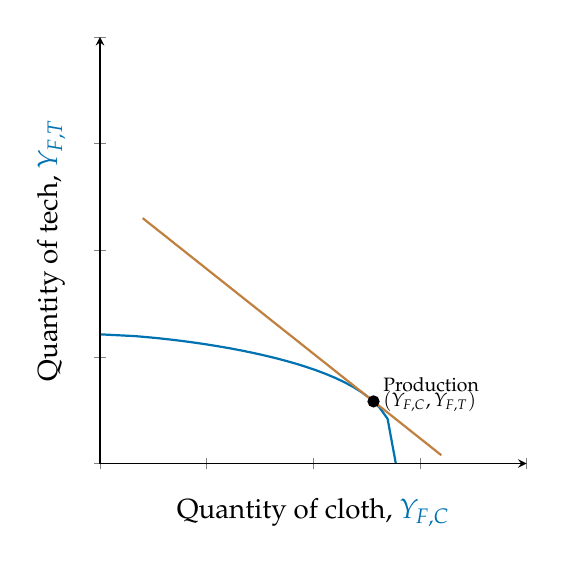
\begin{tikzpicture}
    \pgfmathsetmacro{\alpha}{0.5}
    \pgfmathsetmacro{\betat}{2/3}
    \pgfmathsetmacro{\betac}{1/3}

    \pgfmathsetmacro{\Phi}{((1-\betat)^(1-\betat))*((\betat)^\betat)/
             ((1-\betac)^(1-\betac))*((\betac)^\betac)}
    \pgfmathsetmacro{\aC}{\betac/(1-\betac)}
    \pgfmathsetmacro{\aT}{\betat/(1-\betat)}
    \pgfmathsetmacro{\d}{\aC-\aT}

    
    \pgfmathsetmacro{\L}{2}
    \pgfmathsetmacro{\K}{1}
    \pgfmathsetmacro{\Kk}{1.5}

   \pgfmathsetmacro{\wra}{ \K / \L * (\alpha*(1-\betac) + (1-\alpha)*(1-\betat))/(\alpha * \betac + (1-\alpha)*\betat)  }
    \pgfmathsetmacro{\wr}{  \Kk / \L * (\alpha*(1-\betac) + (1-\alpha)*(1-\betat))/(\alpha * \betac + (1-\alpha)*\betat) }

    \pgfmathsetmacro{\P}{ ( ((1-\betat)^(1-\betat) * \betat^(\betat)) / ((1-\betac)^(1-\betac) * \betac^(\betac)) ) * (\wra)^(\betat-\betac)  }

       
    \pgfmathsetmacro{\Lc}{ (\K - \aT*\wr*\L)/(\d * \wr) }
    \pgfmathsetmacro{\Kc}{\aC * \wr * \Lc}
    \pgfmathsetmacro{\Lt}{\L - \Lc}
    \pgfmathsetmacro{\Kt}{\K - \Kc}
   
    \pgfmathsetmacro{\Yc}{ \Kc^(\betac) * \Lc^(1-\betac) }
    \pgfmathsetmacro{\Yt}{ \Kt^(\betat) * \Lt^(1-\betat) }

    

    \pgfmathsetmacro{\I}{ \P * \Yc + \Yt }
    \pgfmathsetmacro{\Qc}{(1-\alpha)/\P * \I}
    \pgfmathsetmacro{\Qt}{(\alpha) * \I}

    \pgfmathsetmacro{\U}{(\Qt^(\alpha))*(\Qc^(1 - \alpha))}
    \pgfmathsetmacro{\expo}{(1 - \alpha)/\alpha}
    \pgfmathsetmacro{\A}{\U^(1/\alpha)}

    
    
    \centering
    \begin{axis}[
        ylabel={Quantity of tech, $\textcolor{blue}{Y_{F,T}}$},
        xlabel={Quantity of cloth, $\textcolor{blue}{Y_{F,C}}$},
        ymin=0, ymax=2,
        xmin=0, xmax=2,
        yticklabel=\empty,
        xticklabel=\empty,
        axis lines=left,
        enlargelimits=false,
        clip=false,
        axis on top,
        scaled x ticks=false,
        width=7cm, height=7cm,
        title style={font=\bfseries}
    ]
    
    % PPF: Q_C = (L/a_C) - (a_R/a_C) * Q_R
    \addplot[blue, thick, domain=0:2] ({ \Kc^(\betac) * (\L-x)^(1-\betac)}, { \Kt^(\betat) * (x)^(1-\betat)});
    \pgfmathsetmacro{\c}{ \Yt + \P * \Yc }
    \addplot[thick, brown, domain=0.2:1.6] { \c - \P*x};
    

    % Equilibrium point
    \addplot[only marks, mark=*, color=black, mark size=2pt] coordinates {(\Yc, \Yt)};
    \node[anchor = south west] at (axis cs:\Yc,\Yt) {\scriptsize Production};
    \node[anchor = west] at (axis cs:\Yc,\Yt) {\scriptsize $(Y_{F,C},Y_{F,T})$};
        

    
    \end{axis}

\end{tikzpicture}

    \end{column}
\end{columns}
\end{frame}




\begin{frame}{Graphical representation}
\addtocounter{framenumber}{-1}

\begin{columns}[T] % align columns
\begin{column}{.4\textwidth}
            \centering
    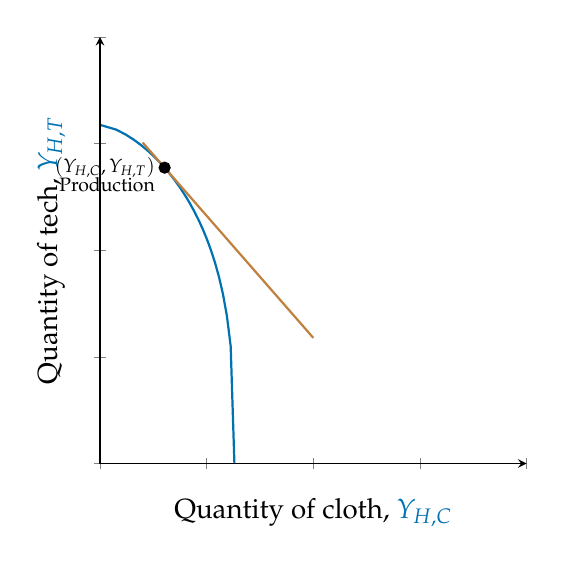
\begin{tikzpicture}
    \pgfmathsetmacro{\alpha}{0.5}
    \pgfmathsetmacro{\betat}{2/3}
    \pgfmathsetmacro{\betac}{1/3}

    \pgfmathsetmacro{\Phi}{((1-\betat)^(1-\betat))*((\betat)^\betat)/
             ((1-\betac)^(1-\betac))*((\betac)^\betac)}
    \pgfmathsetmacro{\aC}{\betac/(1-\betac)}
    \pgfmathsetmacro{\aT}{\betat/(1-\betat)}
    \pgfmathsetmacro{\d}{\aC-\aT}

    
    \pgfmathsetmacro{\L}{1}
    \pgfmathsetmacro{\K}{2.25}
    \pgfmathsetmacro{\Kk}{1.5}

   \pgfmathsetmacro{\wra}{ \K / \L * (\alpha*(1-\betac) + (1-\alpha)*(1-\betat))/(\alpha * \betac + (1-\alpha)*\betat)  }
    \pgfmathsetmacro{\wr}{  \Kk / \L * (\alpha*(1-\betac) + (1-\alpha)*(1-\betat))/(\alpha * \betac + (1-\alpha)*\betat) }

    \pgfmathsetmacro{\P}{ ( ((1-\betat)^(1-\betat) * \betat^(\betat)) / ((1-\betac)^(1-\betac) * \betac^(\betac)) ) * (\wr)^(\betat-\betac)  }

       
    \pgfmathsetmacro{\Lc}{ (\K - \aT*\wr*\L)/(\d * \wr) }
    \pgfmathsetmacro{\Kc}{\aC * \wr * \Lc}
    \pgfmathsetmacro{\Lt}{\L - \Lc}
    \pgfmathsetmacro{\Kt}{\K - \Kc}
   
    \pgfmathsetmacro{\Yc}{ \Kc^(\betac) * \Lc^(1-\betac) }
    \pgfmathsetmacro{\Yt}{ \Kt^(\betat) * \Lt^(1-\betat) }

    

    \pgfmathsetmacro{\I}{ \P * \Yc + \Yt }
    \pgfmathsetmacro{\Qc}{(1-\alpha)/\P * \I}
    \pgfmathsetmacro{\Qt}{(\alpha) * \I}

    \pgfmathsetmacro{\U}{(\Qt^(\alpha))*(\Qc^(1 - \alpha))}
    \pgfmathsetmacro{\expo}{(1 - \alpha)/\alpha}
    \pgfmathsetmacro{\A}{\U^(1/\alpha)}

    
    
    \centering
    \begin{axis}[
        ylabel={Quantity of tech, $\textcolor{blue}{Y_{H,T}}$},
        xlabel={Quantity of cloth, $\textcolor{blue}{Y_{H,C}}$},
        ymin=0, ymax=2,
        xmin=0, xmax=2,
        yticklabel=\empty,
        xticklabel=\empty,
        axis lines=left,
        enlargelimits=false,
        clip=false,
        axis on top,
        scaled x ticks=false,
        width=7cm, height=7cm,
        title style={font=\bfseries}
    ]
    
    % PPF: Q_C = (L/a_C) - (a_R/a_C) * Q_R
    \addplot[blue, thick, domain=0:1] ({ \Kc^(\betac) * (\L-x)^(1-\betac)}, { \Kt^(\betat) * (x)^(1-\betat)});
    \pgfmathsetmacro{\c}{ \Yt + \P * \Yc }
    \addplot[thick, brown, domain=0.2:1] { \c - \P*x};
    

    % Equilibrium point
    \addplot[only marks, mark=*, color=black, mark size=2pt] coordinates {(\Yc, \Yt)};
    \node[anchor = north east] at (axis cs:\Yc,\Yt) {\scriptsize Production};
    \node[anchor = east] at (axis cs:\Yc,\Yt) {\scriptsize $(Y_{H,C},Y_{H,T})$};
        

    
    \end{axis}

\end{tikzpicture}

                
    \end{column}
    \begin{column}{.45\textwidth}

    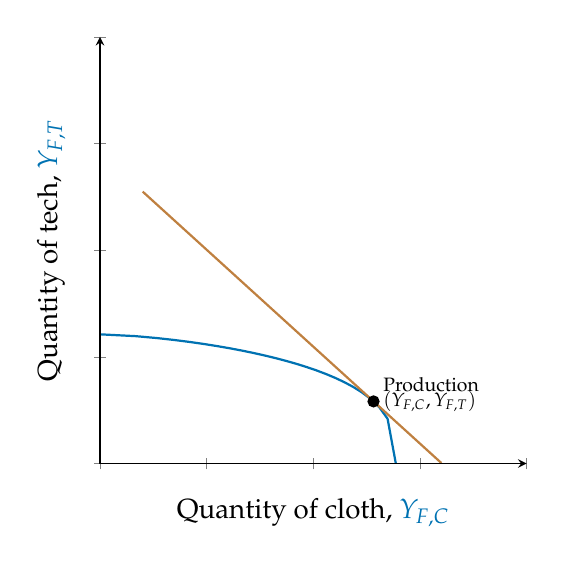
\begin{tikzpicture}
    \pgfmathsetmacro{\alpha}{0.5}
    \pgfmathsetmacro{\betat}{2/3}
    \pgfmathsetmacro{\betac}{1/3}

    \pgfmathsetmacro{\Phi}{((1-\betat)^(1-\betat))*((\betat)^\betat)/
             ((1-\betac)^(1-\betac))*((\betac)^\betac)}
    \pgfmathsetmacro{\aC}{\betac/(1-\betac)}
    \pgfmathsetmacro{\aT}{\betat/(1-\betat)}
    \pgfmathsetmacro{\d}{\aC-\aT}

    
    \pgfmathsetmacro{\L}{2}
    \pgfmathsetmacro{\K}{1}
    \pgfmathsetmacro{\Kk}{1.5}

   \pgfmathsetmacro{\wra}{ \K / \L * (\alpha*(1-\betac) + (1-\alpha)*(1-\betat))/(\alpha * \betac + (1-\alpha)*\betat)  }
    \pgfmathsetmacro{\wr}{  \Kk / \L * (\alpha*(1-\betac) + (1-\alpha)*(1-\betat))/(\alpha * \betac + (1-\alpha)*\betat) }

    \pgfmathsetmacro{\P}{ ( ((1-\betat)^(1-\betat) * \betat^(\betat)) / ((1-\betac)^(1-\betac) * \betac^(\betac)) ) * (\wr)^(\betat-\betac)  }

       
    \pgfmathsetmacro{\Lc}{ (\K - \aT*\wr*\L)/(\d * \wr) }
    \pgfmathsetmacro{\Kc}{\aC * \wr * \Lc}
    \pgfmathsetmacro{\Lt}{\L - \Lc}
    \pgfmathsetmacro{\Kt}{\K - \Kc}
   
    \pgfmathsetmacro{\Yc}{ \Kc^(\betac) * \Lc^(1-\betac) }
    \pgfmathsetmacro{\Yt}{ \Kt^(\betat) * \Lt^(1-\betat) }

    

    \pgfmathsetmacro{\I}{ \P * \Yc + \Yt }
    \pgfmathsetmacro{\Qc}{(1-\alpha)/\P * \I}
    \pgfmathsetmacro{\Qt}{(\alpha) * \I}

    \pgfmathsetmacro{\U}{(\Qt^(\alpha))*(\Qc^(1 - \alpha))}
    \pgfmathsetmacro{\expo}{(1 - \alpha)/\alpha}
    \pgfmathsetmacro{\A}{\U^(1/\alpha)}

    
    
    \centering
    \begin{axis}[
        ylabel={Quantity of tech, $\textcolor{blue}{Y_{F,T}}$},
        xlabel={Quantity of cloth, $\textcolor{blue}{Y_{F,C}}$},
        ymin=0, ymax=2,
        xmin=0, xmax=2,
        yticklabel=\empty,
        xticklabel=\empty,
        axis lines=left,
        enlargelimits=false,
        clip=false,
        axis on top,
        scaled x ticks=false,
        width=7cm, height=7cm,
        title style={font=\bfseries}
    ]
    
    % PPF: Q_C = (L/a_C) - (a_R/a_C) * Q_R
    \addplot[blue, thick, domain=0:2] ({ \Kc^(\betac) * (\L-x)^(1-\betac)}, { \Kt^(\betat) * (x)^(1-\betat)});
    \pgfmathsetmacro{\c}{ \Yt + \P * \Yc }
    \addplot[thick, brown, domain=0.2:1.6] { \c - \P*x};
    

    % Equilibrium point
    \addplot[only marks, mark=*, color=black, mark size=2pt] coordinates {(\Yc, \Yt)};
    \node[anchor = south west] at (axis cs:\Yc,\Yt) {\scriptsize Production};
    \node[anchor = west] at (axis cs:\Yc,\Yt) {\scriptsize $(Y_{F,C},Y_{F,T})$};
        

    
    \end{axis}

\end{tikzpicture}

    \end{column}
\end{columns}
\end{frame}


\begin{frame}{Graphical representation}
\addtocounter{framenumber}{-1}

\begin{columns}[T] % align columns
\begin{column}{.4\textwidth}
            \centering
    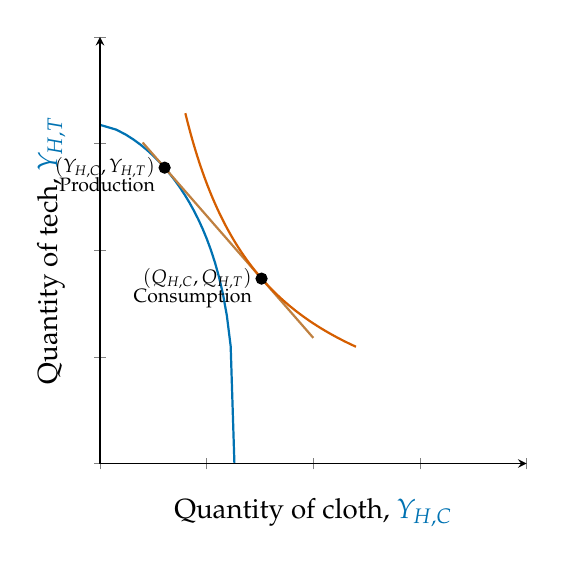
\begin{tikzpicture}
    \pgfmathsetmacro{\alpha}{0.5}
    \pgfmathsetmacro{\betat}{2/3}
    \pgfmathsetmacro{\betac}{1/3}

    \pgfmathsetmacro{\Phi}{((1-\betat)^(1-\betat))*((\betat)^\betat)/
             ((1-\betac)^(1-\betac))*((\betac)^\betac)}
    \pgfmathsetmacro{\aC}{\betac/(1-\betac)}
    \pgfmathsetmacro{\aT}{\betat/(1-\betat)}
    \pgfmathsetmacro{\d}{\aC-\aT}

    
    \pgfmathsetmacro{\L}{1}
    \pgfmathsetmacro{\K}{2.25}
    \pgfmathsetmacro{\Kk}{1.5}

   \pgfmathsetmacro{\wra}{ \K / \L * (\alpha*(1-\betac) + (1-\alpha)*(1-\betat))/(\alpha * \betac + (1-\alpha)*\betat)  }
    \pgfmathsetmacro{\wr}{  \Kk / \L * (\alpha*(1-\betac) + (1-\alpha)*(1-\betat))/(\alpha * \betac + (1-\alpha)*\betat) }

    \pgfmathsetmacro{\P}{ ( ((1-\betat)^(1-\betat) * \betat^(\betat)) / ((1-\betac)^(1-\betac) * \betac^(\betac)) ) * (\wr)^(\betat-\betac)  }

       
    \pgfmathsetmacro{\Lc}{ (\K - \aT*\wr*\L)/(\d * \wr) }
    \pgfmathsetmacro{\Kc}{\aC * \wr * \Lc}
    \pgfmathsetmacro{\Lt}{\L - \Lc}
    \pgfmathsetmacro{\Kt}{\K - \Kc}
   
    \pgfmathsetmacro{\Yc}{ \Kc^(\betac) * \Lc^(1-\betac) }
    \pgfmathsetmacro{\Yt}{ \Kt^(\betat) * \Lt^(1-\betat) }

    

    \pgfmathsetmacro{\I}{ \P * \Yc + \Yt }
    \pgfmathsetmacro{\Qc}{(1-\alpha)/\P * \I}
    \pgfmathsetmacro{\Qt}{(\alpha) * \I}

    \pgfmathsetmacro{\U}{(\Qt^(\alpha))*(\Qc^(1 - \alpha))}
    \pgfmathsetmacro{\expo}{(1 - \alpha)/\alpha}
    \pgfmathsetmacro{\A}{\U^(1/\alpha)}

    
    
    \centering
    \begin{axis}[
        ylabel={Quantity of tech, $\textcolor{blue}{Y_{H,T}}$},
        xlabel={Quantity of cloth, $\textcolor{blue}{Y_{H,C}}$},
        ymin=0, ymax=2,
        xmin=0, xmax=2,
        yticklabel=\empty,
        xticklabel=\empty,
        axis lines=left,
        enlargelimits=false,
        clip=false,
        axis on top,
        scaled x ticks=false,
        width=7cm, height=7cm,
        title style={font=\bfseries}
    ]
    
    % PPF: Q_C = (L/a_C) - (a_R/a_C) * Q_R
    \addplot[blue, thick, domain=0:1] ({ \Kc^(\betac) * (\L-x)^(1-\betac)}, { \Kt^(\betat) * (x)^(1-\betat)});
    \pgfmathsetmacro{\c}{ \Yt + \P * \Yc }
    \addplot[thick, brown, domain=0.2:1] { \c - \P*x};
    
    \addplot[thick, red, domain=0.4:1.2, samples=100] {\A * x^(-\expo)};

    % Equilibrium point
    \addplot[only marks, mark=*, color=black, mark size=2pt] coordinates {(\Yc, \Yt)};
    \node[anchor = north east] at (axis cs:\Yc,\Yt) {\scriptsize Production};
    \node[anchor = east] at (axis cs:\Yc,\Yt) {\scriptsize $(Y_{H,C},Y_{H,T})$};
        
    \addplot[only marks, mark=*, color=black, mark size=2pt] coordinates {(\Qc, \Qt)};
    \node[anchor = north east] at (axis cs:\Qc,\Qt) {\scriptsize Consumption};
    \node[anchor = east] at (axis cs:\Qc,\Qt) {\scriptsize $(Q_{H,C},Q_{H,T})$};

    
    \end{axis}

\end{tikzpicture}

                
    \end{column}
    \begin{column}{.45\textwidth}

    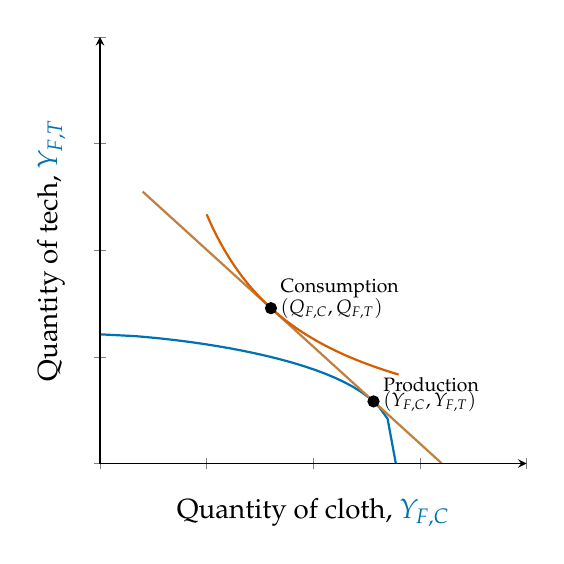
\begin{tikzpicture}
    \pgfmathsetmacro{\alpha}{0.5}
    \pgfmathsetmacro{\betat}{2/3}
    \pgfmathsetmacro{\betac}{1/3}

    \pgfmathsetmacro{\Phi}{((1-\betat)^(1-\betat))*((\betat)^\betat)/
             ((1-\betac)^(1-\betac))*((\betac)^\betac)}
    \pgfmathsetmacro{\aC}{\betac/(1-\betac)}
    \pgfmathsetmacro{\aT}{\betat/(1-\betat)}
    \pgfmathsetmacro{\d}{\aC-\aT}

    
    \pgfmathsetmacro{\L}{2}
    \pgfmathsetmacro{\K}{1}
    \pgfmathsetmacro{\Kk}{1.5}

   \pgfmathsetmacro{\wra}{ \K / \L * (\alpha*(1-\betac) + (1-\alpha)*(1-\betat))/(\alpha * \betac + (1-\alpha)*\betat)  }
    \pgfmathsetmacro{\wr}{  \Kk / \L * (\alpha*(1-\betac) + (1-\alpha)*(1-\betat))/(\alpha * \betac + (1-\alpha)*\betat) }

    \pgfmathsetmacro{\P}{ ( ((1-\betat)^(1-\betat) * \betat^(\betat)) / ((1-\betac)^(1-\betac) * \betac^(\betac)) ) * (\wr)^(\betat-\betac)  }

       
    \pgfmathsetmacro{\Lc}{ (\K - \aT*\wr*\L)/(\d * \wr) }
    \pgfmathsetmacro{\Kc}{\aC * \wr * \Lc}
    \pgfmathsetmacro{\Lt}{\L - \Lc}
    \pgfmathsetmacro{\Kt}{\K - \Kc}
   
    \pgfmathsetmacro{\Yc}{ \Kc^(\betac) * \Lc^(1-\betac) }
    \pgfmathsetmacro{\Yt}{ \Kt^(\betat) * \Lt^(1-\betat) }

    

    \pgfmathsetmacro{\I}{ \P * \Yc + \Yt }
    \pgfmathsetmacro{\Qc}{(1-\alpha)/\P * \I}
    \pgfmathsetmacro{\Qt}{(\alpha) * \I}

    \pgfmathsetmacro{\U}{(\Qt^(\alpha))*(\Qc^(1 - \alpha))}
    \pgfmathsetmacro{\expo}{(1 - \alpha)/\alpha}
    \pgfmathsetmacro{\A}{\U^(1/\alpha)}

    
    
    \centering
    \begin{axis}[
        ylabel={Quantity of tech, $\textcolor{blue}{Y_{F,T}}$},
        xlabel={Quantity of cloth, $\textcolor{blue}{Y_{F,C}}$},
        ymin=0, ymax=2,
        xmin=0, xmax=2,
        yticklabel=\empty,
        xticklabel=\empty,
        axis lines=left,
        enlargelimits=false,
        clip=false,
        axis on top,
        scaled x ticks=false,
        width=7cm, height=7cm,
        title style={font=\bfseries}
    ]
    
    % PPF: Q_C = (L/a_C) - (a_R/a_C) * Q_R
    \addplot[blue, thick, domain=0:2] ({ \Kc^(\betac) * (\L-x)^(1-\betac)}, { \Kt^(\betat) * (x)^(1-\betat)});
    \pgfmathsetmacro{\c}{ \Yt + \P * \Yc }
    \addplot[thick, brown, domain=0.2:1.6] { \c - \P*x};
    
    \addplot[thick, red, domain=0.5:1.4, samples=100] {\A * x^(-\expo)};

    % Equilibrium point
    \addplot[only marks, mark=*, color=black, mark size=2pt] coordinates {(\Yc, \Yt)};
    \node[anchor = south west] at (axis cs:\Yc,\Yt) {\scriptsize Production};
    \node[anchor = west] at (axis cs:\Yc,\Yt) {\scriptsize $(Y_{F,C},Y_{F,T})$};
        
    \addplot[only marks, mark=*, color=black, mark size=2pt] coordinates {(\Qc, \Qt)};
    \node[anchor = south west] at (axis cs:\Qc,\Qt) {\scriptsize Consumption};
    \node[anchor = west] at (axis cs:\Qc,\Qt) {\scriptsize $(Q_{F,C},Q_{F,T})$};

    
    \end{axis}

\end{tikzpicture}

    \end{column}
\end{columns}
\end{frame}

\begin{frame}{Graphical representation}
\addtocounter{framenumber}{-1}

\begin{columns}[T] % align columns
\begin{column}{.4\textwidth}
            \centering
    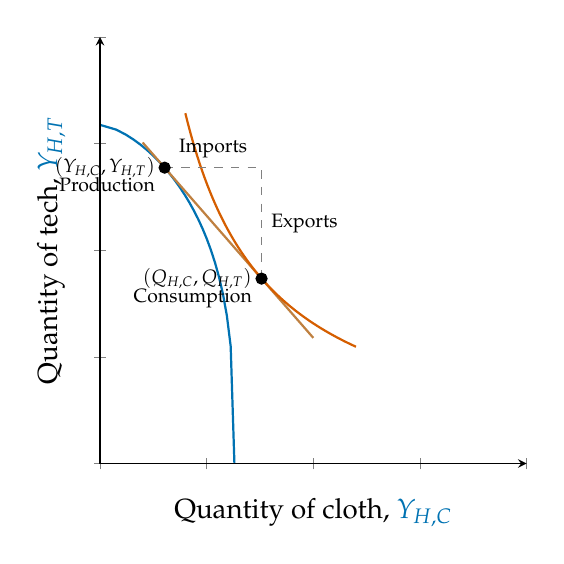
\begin{tikzpicture}
    \pgfmathsetmacro{\alpha}{0.5}
    \pgfmathsetmacro{\betat}{2/3}
    \pgfmathsetmacro{\betac}{1/3}

    \pgfmathsetmacro{\Phi}{((1-\betat)^(1-\betat))*((\betat)^\betat)/
             ((1-\betac)^(1-\betac))*((\betac)^\betac)}
    \pgfmathsetmacro{\aC}{\betac/(1-\betac)}
    \pgfmathsetmacro{\aT}{\betat/(1-\betat)}
    \pgfmathsetmacro{\d}{\aC-\aT}

    
    \pgfmathsetmacro{\L}{1}
    \pgfmathsetmacro{\K}{2.25}
    \pgfmathsetmacro{\Kk}{1.5}

   \pgfmathsetmacro{\wra}{ \K / \L * (\alpha*(1-\betac) + (1-\alpha)*(1-\betat))/(\alpha * \betac + (1-\alpha)*\betat)  }
    \pgfmathsetmacro{\wr}{  \Kk / \L * (\alpha*(1-\betac) + (1-\alpha)*(1-\betat))/(\alpha * \betac + (1-\alpha)*\betat) }

    \pgfmathsetmacro{\P}{ ( ((1-\betat)^(1-\betat) * \betat^(\betat)) / ((1-\betac)^(1-\betac) * \betac^(\betac)) ) * (\wr)^(\betat-\betac)  }

       
    \pgfmathsetmacro{\Lc}{ (\K - \aT*\wr*\L)/(\d * \wr) }
    \pgfmathsetmacro{\Kc}{\aC * \wr * \Lc}
    \pgfmathsetmacro{\Lt}{\L - \Lc}
    \pgfmathsetmacro{\Kt}{\K - \Kc}
   
    \pgfmathsetmacro{\Yc}{ \Kc^(\betac) * \Lc^(1-\betac) }
    \pgfmathsetmacro{\Yt}{ \Kt^(\betat) * \Lt^(1-\betat) }

    

    \pgfmathsetmacro{\I}{ \P * \Yc + \Yt }
    \pgfmathsetmacro{\Qc}{(1-\alpha)/\P * \I}
    \pgfmathsetmacro{\Qt}{(\alpha) * \I}

    \pgfmathsetmacro{\U}{(\Qt^(\alpha))*(\Qc^(1 - \alpha))}
    \pgfmathsetmacro{\expo}{(1 - \alpha)/\alpha}
    \pgfmathsetmacro{\A}{\U^(1/\alpha)}

    
    
    \centering
    \begin{axis}[
        ylabel={Quantity of tech, $\textcolor{blue}{Y_{H,T}}$},
        xlabel={Quantity of cloth, $\textcolor{blue}{Y_{H,C}}$},
        ymin=0, ymax=2,
        xmin=0, xmax=2,
        yticklabel=\empty,
        xticklabel=\empty,
        axis lines=left,
        enlargelimits=false,
        clip=false,
        axis on top,
        scaled x ticks=false,
        width=7cm, height=7cm,
        title style={font=\bfseries}
    ]
    
    % PPF: Q_C = (L/a_C) - (a_R/a_C) * Q_R
    \addplot[blue, thick, domain=0:1] ({ \Kc^(\betac) * (\L-x)^(1-\betac)}, { \Kt^(\betat) * (x)^(1-\betat)});
    \pgfmathsetmacro{\c}{ \Yt + \P * \Yc }
    \addplot[thick, brown, domain=0.2:1] { \c - \P*x};
    
    \addplot[thick, red, domain=0.4:1.2, samples=100] {\A * x^(-\expo)};

    % Equilibrium point
    \addplot[only marks, mark=*, color=black, mark size=2pt] coordinates {(\Yc, \Yt)};
    \node[anchor = north east] at (axis cs:\Yc,\Yt) {\scriptsize Production};
    \node[anchor = east] at (axis cs:\Yc,\Yt) {\scriptsize $(Y_{H,C},Y_{H,T})$};
        
    \addplot[only marks, mark=*, color=black, mark size=2pt] coordinates {(\Qc, \Qt)};
    \node[anchor = north east] at (axis cs:\Qc,\Qt) {\scriptsize Consumption};
    \node[anchor = east] at (axis cs:\Qc,\Qt) {\scriptsize $(Q_{H,C},Q_{H,T})$};

    \addplot[dashed, gray] coordinates {(\Yc, \Yt) (\Qc, \Yt)  (\Qc, \Qt)};
    \node[anchor = south] at (axis cs:{\Yc + (\Qc-\Yc)/2}, \Yt) {\scriptsize Imports};
    \node[anchor = west] at (axis cs:\Qc, {\Yt + (\Qt-\Yt)/2}) {\scriptsize Exports};
    
    \end{axis}

\end{tikzpicture}

                
    \end{column}
    \begin{column}{.45\textwidth}

    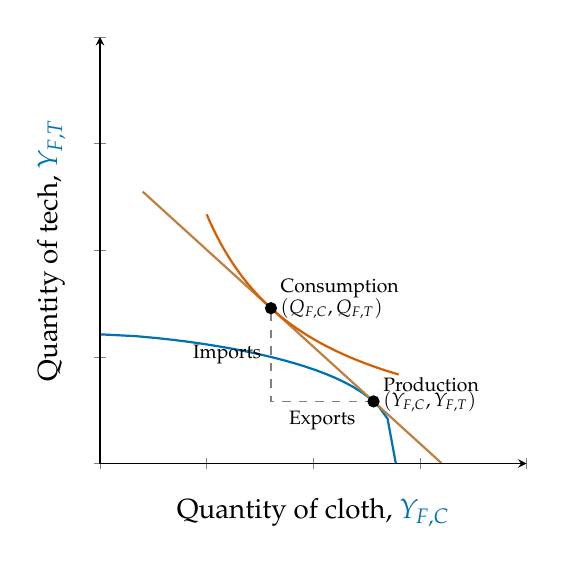
\begin{tikzpicture}
    \pgfmathsetmacro{\alpha}{0.5}
    \pgfmathsetmacro{\betat}{2/3}
    \pgfmathsetmacro{\betac}{1/3}

    \pgfmathsetmacro{\Phi}{((1-\betat)^(1-\betat))*((\betat)^\betat)/
             ((1-\betac)^(1-\betac))*((\betac)^\betac)}
    \pgfmathsetmacro{\aC}{\betac/(1-\betac)}
    \pgfmathsetmacro{\aT}{\betat/(1-\betat)}
    \pgfmathsetmacro{\d}{\aC-\aT}

    
    \pgfmathsetmacro{\L}{2}
    \pgfmathsetmacro{\K}{1}
    \pgfmathsetmacro{\Kk}{1.5}

   \pgfmathsetmacro{\wra}{ \K / \L * (\alpha*(1-\betac) + (1-\alpha)*(1-\betat))/(\alpha * \betac + (1-\alpha)*\betat)  }
    \pgfmathsetmacro{\wr}{  \Kk / \L * (\alpha*(1-\betac) + (1-\alpha)*(1-\betat))/(\alpha * \betac + (1-\alpha)*\betat) }

    \pgfmathsetmacro{\P}{ ( ((1-\betat)^(1-\betat) * \betat^(\betat)) / ((1-\betac)^(1-\betac) * \betac^(\betac)) ) * (\wr)^(\betat-\betac)  }

       
    \pgfmathsetmacro{\Lc}{ (\K - \aT*\wr*\L)/(\d * \wr) }
    \pgfmathsetmacro{\Kc}{\aC * \wr * \Lc}
    \pgfmathsetmacro{\Lt}{\L - \Lc}
    \pgfmathsetmacro{\Kt}{\K - \Kc}
   
    \pgfmathsetmacro{\Yc}{ \Kc^(\betac) * \Lc^(1-\betac) }
    \pgfmathsetmacro{\Yt}{ \Kt^(\betat) * \Lt^(1-\betat) }

    

    \pgfmathsetmacro{\I}{ \P * \Yc + \Yt }
    \pgfmathsetmacro{\Qc}{(1-\alpha)/\P * \I}
    \pgfmathsetmacro{\Qt}{(\alpha) * \I}

    \pgfmathsetmacro{\U}{(\Qt^(\alpha))*(\Qc^(1 - \alpha))}
    \pgfmathsetmacro{\expo}{(1 - \alpha)/\alpha}
    \pgfmathsetmacro{\A}{\U^(1/\alpha)}

    
    
    \centering
    \begin{axis}[
        ylabel={Quantity of tech, $\textcolor{blue}{Y_{F,T}}$},
        xlabel={Quantity of cloth, $\textcolor{blue}{Y_{F,C}}$},
        ymin=0, ymax=2,
        xmin=0, xmax=2,
        yticklabel=\empty,
        xticklabel=\empty,
        axis lines=left,
        enlargelimits=false,
        clip=false,
        axis on top,
        scaled x ticks=false,
        width=7cm, height=7cm,
        title style={font=\bfseries}
    ]
    
    % PPF: Q_C = (L/a_C) - (a_R/a_C) * Q_R
    \addplot[blue, thick, domain=0:2] ({ \Kc^(\betac) * (\L-x)^(1-\betac)}, { \Kt^(\betat) * (x)^(1-\betat)});
    \pgfmathsetmacro{\c}{ \Yt + \P * \Yc }
    \addplot[thick, brown, domain=0.2:1.6] { \c - \P*x};
    
    \addplot[thick, red, domain=0.5:1.4, samples=100] {\A * x^(-\expo)};

    % Equilibrium point
    \addplot[only marks, mark=*, color=black, mark size=2pt] coordinates {(\Yc, \Yt)};
    \node[anchor = south west] at (axis cs:\Yc,\Yt) {\scriptsize Production};
    \node[anchor = west] at (axis cs:\Yc,\Yt) {\scriptsize $(Y_{F,C},Y_{F,T})$};
        
    \addplot[only marks, mark=*, color=black, mark size=2pt] coordinates {(\Qc, \Qt)};
    \node[anchor = south west] at (axis cs:\Qc,\Qt) {\scriptsize Consumption};
    \node[anchor = west] at (axis cs:\Qc,\Qt) {\scriptsize $(Q_{F,C},Q_{F,T})$};

    \addplot[dashed, gray] coordinates {(\Yc, \Yt) (\Qc, \Yt)  (\Qc, \Qt)};
    \node[anchor = north] at (axis cs:{\Yc + (\Qc-\Yc)/2}, \Yt) {\scriptsize Exports};
    \node[anchor = east] at (axis cs:\Qc, {\Yt + (\Qt-\Yt)/2}) {\scriptsize Imports};
    
    \end{axis}

\end{tikzpicture}

    \end{column}
\end{columns}
\end{frame}


\section{STM: Different Preferences}

\section{STM: Different Technologies}


\begin{frame}{Key STM objects and notation}
\begin{wideitemize}
  \item Two goods: $C$ (cloth) and $T$ (tech/food). Relative price: $p \equiv P_C/P_T$
  \item Domestic \textbf{relative supply:} $RS(p) \equiv \frac{Q_C(p)}{Q_T(p)}$
  \item Domestic \textbf{relative demand:} $RD(p) \equiv \frac{D_C(p,Y)}{D_T(p,Y)}$
  \item World equilibrium: $p^{w}$ s.t. $RS^{\text{world}}(p^{w})=RD^{\text{world}}(p^{w})$
  \item Terms of Trade (Home): $\text{ToT}_H = \frac{P_{\text{exports}}}{P_{\text{imports}}}$
\end{wideitemize}
\end{frame}

\begin{frame}{From PPF to RS}
\begin{columns}[T]
\begin{column}{0.58\textwidth}
\begin{wideitemize}
  \item Producer chooses $(Q_C,Q_T)$ to maximize $P_C Q_C + P_T Q_T$ over the PPF
  \item Slope at optimum: $MRT_{C,T} = \frac{dQ_T}{dQ_C} = -\frac{P_C}{P_T}=-p$
  \item As $p$ rises, production tilts to $C$ $\Rightarrow$ \textbf{RS is upward sloping}
  \item With kinks (specialization), RS has flat segments/jumps
\end{wideitemize}
\end{column}
\begin{column}{0.38\textwidth}
\centering
%\includegraphics[width=\linewidth]{figs/ppf_tangency_to_isorevenue.pdf}\\[2mm]
%\includegraphics[width=\linewidth]{figs/domestic_RS_from_ppf.pdf}
\end{column}
\end{columns}
\end{frame}

\begin{frame}{From preferences to RD}
\begin{columns}[T]
\begin{column}{0.58\textwidth}
\begin{wideitemize}
  \item Consumer chooses $(D_C,D_T)$ to maximize $U(C,T)$ s.t. $P_C D_C + P_T D_T = Y$
  \item As $p$ rises, $C$ becomes relatively expensive $\Rightarrow$ \textbf{RD falls} in $p$
  \item With homothetic preferences, $RD(p)$ does not shift with $Y$ (only with tastes)
  \item Example (CES with elasticity $\sigma$):
  \[
    RD(p)=\frac{D_C}{D_T}
      =\frac{\alpha}{1-\alpha}\,p^{-\sigma}
  \]
\end{wideitemize}
\end{column}
\begin{column}{0.38\textwidth}
\centering
%\includegraphics[width=\linewidth]{figs/domestic_RD_curve.pdf}
\end{column}
\end{columns}
\end{frame}

\begin{frame}{Domestic equilibrium and gains from trade}
\begin{columns}[T]
\begin{column}{0.58\textwidth}
\begin{wideitemize}
  \item \textbf{Autarky:} $p^A$ at $RS(p)=RD(p)$
  \item \textbf{With trade:} price $p^w$ pins production at RS and consumption on budget line with slope $-p^w$
  \item \textbf{Gains:} trade moves consumption to higher indifference curve if $p^w \neq p^A$
\end{wideitemize}
\end{column}
\begin{column}{0.38\textwidth}
\centering
%\includegraphics[width=\linewidth]{figs/autarky_RS_RD.pdf}\\[2mm]
%\includegraphics[width=\linewidth]{figs/trade_budget_and_IC.pdf}
\end{column}
\end{columns}
\end{frame}

\begin{frame}{World RS and RD}
\begin{wideitemize}
  \item \textbf{World RS:} (roughly) horizontal aggregation of country supplies $\Rightarrow RS^{W}(p)$ is upward sloping with plateaus at specialization ranges
  \item \textbf{World RD:} aggregation of demands; with homothetic preferences, same shape as domestic RD
  \item \textbf{World price $p^w$:} intersection $RS^{W}(p)$ and $RD^{W}(p)$
\end{wideitemize}
\vspace{2mm}
\centering
%\includegraphics[width=0.7\textwidth]{figs/world_RS_RD_equilibrium.pdf}
\end{frame}

\begin{frame}{Shocks in the STM: what moves what?}
\begin{wideitemize}
  \item \textbf{Biased growth in Home}
    \begin{itemize}
      \item Export-biased (toward $C$) $\Rightarrow$ shifts $RS_H$ out in $C$ direction $\Rightarrow$ tends to \emph{lower} $p^w$ (worsen Home ToT)
      \item Import-biased $\Rightarrow$ tends to \emph{raise} $p^w$ (improve Home ToT)
    \end{itemize}
  \item \textbf{Foreign shocks} (growth, policy, preference) shift $RS^W$/$RD^W$ and thus $p^w$
  \item \textbf{Rare case:} Immiserizing growth if ToT deterioration outweighs production gains (needs very steep RD and big growth)
\end{wideitemize}
\end{frame}

\begin{frame}{Trade policies in the STM (large country intuition)}
\begin{wideitemize}
  \item \textbf{Tariff on imports:} raises domestic relative price of import good $\Rightarrow$ moves along RS/RD; for a \emph{large} country, can improve ToT but creates deadweight loss
  \item \textbf{Export subsidy:} reduces ToT (foreign price falls for our export good); always welfare-reducing under standard assumptions
  \item \textbf{Quantifying effects} needs elasticities $\Rightarrow$ gravity (next)
\end{wideitemize}
\end{frame}

% ---------------------------
% Gravity — Concepts
% ---------------------------

\begin{frame}{Gravity: Physics vs. Economics}
\begin{columns}[T]
\begin{column}{0.48\textwidth}
\textbf{Newton's Law of Gravitation}
\[
F_{ij} \;=\; G\,\frac{m_i\,m_j}{r_{ij}^{\,2}}
\]
\begin{wideitemize}
  \item $m_i, m_j$: physical masses
  \item $r_{ij}$: distance between objects
  \item $G$: universal gravitational constant
\end{wideitemize}
\end{column}
\begin{column}{0.48\textwidth}
\textbf{Trade Gravity (reduced form)}
\[
X_{ij} \;=\; K \,\frac{Y_i\,Y_j}{d_{ij}^{\,\theta}}
\]
\begin{wideitemize}
  \item $Y_i, Y_j$: \emph{economic masses} (GDP/total expenditure)
  \item $d_{ij}$: bilateral distance (proxy for trade costs)
  \item $\theta>0$: trade‐cost elasticity (empirical)
  \item $K$: scaling constant / fixed effects
\end{wideitemize}
\end{column}
\end{columns}
\end{frame}

\begin{frame}{From DFS with trade costs to a gravity equation (setup)}
\small
\textbf{Environment (DFS):}
\begin{wideitemize}
  \item Two countries $i,j$; unit interval of goods $g\in[0,1]$ ordered by comparative advantage. Technology summarized by $A_g \equiv a_{j,g}/a_{i,g}$, strictly decreasing in $g$. {\footnotesize (sorting \& unit costs) } \,\,\textit{Pg = min\{$w_i a_{i,g},\, w_j a_{j,g}$\}}.  \,\,{\scriptsize \textcolor{gray}}
  \item Iceberg trade costs $\tau_{ij}>1$: one unit delivered requires $\tau_{ij}$ shipped. {\scriptsize  }
  \item Identical, homothetic (equal-weight) preferences $\Rightarrow$ constant spending density over the unit interval of goods. {\scriptsize \textcolor{gray}}
\end{wideitemize}

\textbf{Export condition:} $i$ is the cheapest \emph{at destination $j$} iff
\[
\tau_{ij}\,w_i a_{i,g} \;\le\; w_j a_{j,g}
\quad\Longleftrightarrow\quad
A_g \;\equiv\; \frac{a_{j,g}}{a_{i,g}} \;\ge\; \tau_{ij}\,\frac{w_i}{w_j}.
\]
Thus $i$ sells to $j$ all goods with $A_g$ above a cutoff; equivalently, $j$ buys from $i$ a share of goods
\[
s_{ij} \;=\; \Pr\!\left[A_g \ge \tau_{ij}\frac{w_i}{w_j}\right].
\]
{\scriptsize \textcolor{gray}{(Trade-cost inequalities and export cutoffs) }}

\textbf{Value of imports by $j$ from $i$:}
\[
X_{ij} \;=\; s_{ij}\,E_j,\qquad \text{with }E_j=w_j L_j \text{ (national expenditure/income).}
\]
{\scriptsize \textcolor{gray}{(balanced spending across goods; income/expenditure identity)}}

\end{frame}

\begin{frame}{A one-line gravity from DFS (Pareto trick)}
\small
\textbf{Assumption on technology dispersion (for tractability):}
Let the relative productivity $A_g$ have a Pareto tail with shape $\theta>0$:
\[
\Pr[A_g \ge a] = a^{-\theta}\quad \text{for } a\ge 1.
\]
Then the export \emph{share} of goods that $i$ sells to $j$ is
\[
s_{ij}=\Pr\!\left[A_g \ge \tau_{ij}\frac{w_i}{w_j}\right]
= \big(\tau_{ij}\tfrac{w_i}{w_j}\big)^{-\theta}.
\]
\textbf{Trade flow:}
\[
\boxed{\,X_{ij} \;=\; E_j\;\tau_{ij}^{-\theta}\;\Big(\frac{w_i}{w_j}\Big)^{-\theta}\,}
\quad\text{with } E_j=w_j L_j.
\]

\textbf{From structure to empirical gravity:}
\begin{wideitemize}
  \item Set $\tau_{ij}=d_{ij}^{\kappa}\times\text{(other frictions)} \;\Rightarrow\; X_{ij}\propto d_{ij}^{-\kappa\theta}$. 
  \item Relative wages $w_i/w_j$ (which in DFS adjust to clear trade and depend on global cutoffs) are absorbed by exporter/importer fixed effects; with many partners this is the “multilateral resistance” idea. So in practice:
  \[
  X_{ij} \;=\; \underbrace{\phi_i}_{\text{exp.\ FE}} \;\underbrace{\psi_j}_{\text{imp.\ FE}}\; d_{ij}^{-\kappa\theta}\;\times\;(\text{observable cost shifters}) .
  \]
  \item Normalizing $\phi_i\propto Y_i$ and $\psi_j\propto Y_j$ yields the classroom gravity form 
  $X_{ij}=K\,\dfrac{Y_i Y_j}{d_{ij}^{\,\theta^\prime}}$ with $\theta^\prime=\kappa\theta$.
\end{wideitemize}

\end{frame}

\begin{frame}{Why gravity?}
\begin{wideitemize}
  \item Connects trade flows to economic size and trade costs
  \item \textbf{Workhorse} for counterfactuals (tariffs, borders, infrastructure) and for mapping STM shocks to data
\end{wideitemize}
\end{frame}

\begin{frame}{Structural gravity (Anderson–van Wincoop)}
\begin{wideitemize}
  \item \textbf{Theory-consistent form:}
  \[
   X_{ij}=\frac{Y_i\,E_j}{Y_W}\left(\frac{\tau_{ij}}{\Pi_i P_j}\right)^{1-\sigma}
  \]
  where $Y_i$ is production, $E_j$ expenditure, $\tau_{ij}$ bilateral costs, $\sigma$ elasticity of substitution,
  $\Pi_i$ outward MR, $P_j$ inward MR.
  \item \textbf{Empirical implementation (PPML):}
  \[
   X_{ij}=\exp\!\left[\beta_1\ln \text{dist}_{ij}+\beta_2\text{border}_{ij}+\cdots
   + \delta^{S}_{i} + \delta^{D}_{j}\right]+\varepsilon_{ij}
  \]
  with exporter and importer (often exporter-year/importer-year) fixed effects absorbing $Y_i, E_j$ and MR terms.
\end{wideitemize}
\end{frame}

\begin{frame}{Gravity: estimation notes (for Data Lab)}
\begin{wideitemize}
  \item \textbf{Use PPML}, not OLS on $\ln X_{ij}$: handles zeros and heteroskedasticity
  \item Include \textbf{high-dimensional FEs}: exporter-year and importer-year (or 3-way when panel)
  \item Standard cost proxies: $\ln$ distance, contiguity, common language, colonial ties, RTA, WTO, tariffs, NTMs
  \item \textbf{Elasticity of trade costs:} $1-\sigma$ scales coefficients; to back out $\sigma$ use separate price/markups or literature priors
\end{wideitemize}
\end{frame}

% ---------------------------
% Applications (intuition)
% ---------------------------
\begin{frame}{Putting STM $\rightarrow$ gravity together}
\begin{wideitemize}
  \item A \textbf{Home export-biased productivity shock} shifts $RS_H$ right
  \item World $p^w$ falls for export good (ToT $\downarrow$ for Home)
  \item In gravity, $\tau_{ij}$ proxies (infrastructure, RTAs, tariffs) shift bilateral $X_{ij}$
  \item Combine: use gravity to \textbf{measure elasticities}, then map STM shocks to quantitative changes in $X_{ij}$ and welfare
\end{wideitemize}
\end{frame}

\begin{frame}{In-class exercise (short)}
\begin{wideitemize}
  \item Sketch $RS$/$RD$ for a country with:
  \begin{itemize}
    \item (i) HO endowments that favor $C$; (ii) preferences CES with $\sigma>1$
  \end{itemize}
  \item Identify autarky $p^A$. Suppose world $p^w>p^A$. Mark production, consumption, and trade bundle.
  \item Now apply a small import tariff on $T$. Show production and consumption wedges and discuss ToT vs. DWL.
\end{wideitemize}
\end{frame}

\begin{frame}{What to remember}
\begin{wideitemize}
  \item STM unifies technology/endowments + preferences via $RS$–$RD$
  \item ToT is the critical link from world prices to welfare
  \item Gravity is the empirical bridge: it maps frictions to flows (and elasticities) for policy counterfactuals
\end{wideitemize}
\end{frame}

% ---------------------------
% (Optional) Appendix slides
% ---------------------------
\begin{frame}{Appendix: quick algebra (CES demand)}
\small
With CES utility $U=\left[\alpha C^{\frac{\sigma-1}{\sigma}}+(1-\alpha)T^{\frac{\sigma-1}{\sigma}}\right]^{\frac{\sigma}{\sigma-1}}$ and income $Y$:
\[
  D_C=\alpha \left(\frac{P_C}{P}\right)^{-\sigma}\frac{Y}{P_C},\quad
  D_T=(1-\alpha)\left(\frac{P_T}{P}\right)^{-\sigma}\frac{Y}{P_T}
\]
\[
  RD(p)=\frac{D_C}{D_T}=\frac{\alpha}{1-\alpha}\,p^{-\sigma}
\]
\end{frame}

\begin{frame}{Appendix: welfare and ToT (Home)}
\small
\begin{wideitemize}
  \item Welfare increases if a shock raises the budget line at the chosen consumption (higher $p^w$ for export good, holding PPF)
  \item Large-country tariff: first-order ToT gain vs. second-order efficiency loss $\Rightarrow$ optimal tariff $\propto 1/\varepsilon^{*}$ (foreign export supply elasticity)
\end{wideitemize}
\end{frame}


\end{document}
